In Ch.~\ref{ch:latticeqcd}, we saw that calculating two-point correlation functions on the lattice using the Monte Carlo method involves evaluating some function of the inverse of the Dirac matrix, i.e.\ some function of the quark propagator. The task of inverting the Dirac matrix is a formidable one. The Dirac matrix carries indices for spacetime, color, and Dirac spin, so for a theory of three colors and four Dirac indices on a $32^3\times 256$ lattice, this amounts to a complex-valued matrix of size $\sim 10^8\times 10^8$. Storing such a matrix in single precision would take roughly 80 petabytes, and so calculating the inverse directly is obvious unfeasible. In this chapter we will discuss methods to tackle this problem that involve stochastically estimating Dirac matrix inverses. We will see that the path integration over the quark fields can be done analytically, but it results in a complicated expression involving the gluon field. The path integration over the gluon field must be estimated using Monte Carlo methods.
\section{Quark Lines}
Calculating a correlator on the lattice involves integrating first over quark fields which are complex Grassmann valued. Recall from Ch.~\ref{ch:latticeqcd} that such an integration results in some function $f$ of the Dirac matrix inverse and the determinant of the Dirac matrix. For example, a meson correlator involves an integral of the form
\begin{equation}
    \int \mathcal{D}[\overline{\psi}, \psi] \psi_{a} \psi_{b} \overline{\psi}_{c} \overline{\psi}_{d} \exp \left(-\overline{\psi}^{T} M \psi\right) = \left(M_{a d}^{-1} M_{b c}^{-1}-M_{a c}^{-1} M_{b d}^{-1}\right) \det M,
\end{equation}
and a baryonic correlator inolves an integral of the form
\begin{eqnarray}
    &&\int {\cal D}[\overline{\psi},\psi]\ \psi_{a_1}\psi_{a_2}\psi_{a_3}
       \ \overline{\psi}_{b_1}\overline{\psi}_{b_2}\overline{\psi}_{b_3}
     \ \exp\left( -\overline{\psi}^T M \psi \right)\nonumber\\
     &=&\biggl( - M_{a_1b_1}^{-1}M^{-1}_{a_2b_2}M^{-1}_{a_3b_3}
     +M^{-1}_{a_1b_1}M^{-1}_{a_2b_3}M^{-1}_{a_3b_2}
      +M^{-1}_{a_1b_2}M^{-1}_{a_2b_1}M^{-1}_{a_3b_3} \nonumber\\
    && \phantom{\biggl(}-M_{a_1b_2}^{-1}M^{-1}_{a_2b_3}M^{-1}_{a_3b_1}
     -M^{-1}_{a_1b_3}M^{-1}_{a_2b_1}M^{-1}_{a_3b_2}
      +M^{-1}_{a_1b_3}M^{-1}_{a_2b_2}M^{-1}_{a_3b_1}   
      \biggr)\ \det M.
      \label{eq:barywick}
\end{eqnarray}
In general, including the fact that our quark fields are smeared and covariantly displaced, so the Grassmann integrals we need to compute are really of the form
\begin{equation}
    \int \mathcal{D}[\chi, \psi] \sum_{\alpha d} f_{a c} \psi_{c} \chi_{d} g_{d b} \exp \left(-\chi^{T} \Omega \psi\right)=\sum_{c d} f_{a c} \Omega_{c d}^{-1} g_{d b} \operatorname{det} \Omega,
\end{equation}
where we have made the substitutions $\chi \equiv \overline \psi \gamma_4$ and $\Omega = \gamma_4 M$, and where $f_{ac}$ and $g_{db}$ are $c$-number coefficients. Each factor of $\Omega^{-1}$ is referred to as a \emph{quark line}. When computing temporal correlators, we can classify quark lines as follows:
\begin{itemize}
    \item forward-time quark lines originate from $\chi$ at a time $t_0$ and terminate to $\psi$ at a later time $t$
    \item backward-time quark lines originate from $\chi$ at a time $t$ and terminate to $\psi$ at an earlier time $t_0$
    \item same-time quark lines originate from $\chi$ and terminate to $\psi$ at the same time, either $t$ or $t_0$.
\end{itemize}
In a two-point correlator, $t_0$ is referred to as the \emph{source time} and $t$ is referred to as the \emph{sink time}. These different types of quark lines are depicted in Fig.~\ref{fig:quark_lines}. Recall the definition of the smearing operator $\mathcal S$ from Eq.~(\ref{eq:smearing_operator}) and the covariant displacement operator $D$ from Eq.~(\ref{eq:displacement_operator}). The quark lines we work with in practice arise from smeared and displaced quark and antiquark fields, so we refer to
\begin{equation}
    (D_{j})_{a b} \mathcal{S}_{b c} \Omega_{c h}^{-1} \mathcal{S}_{h g}(D_{k}^{\dagger})_{g f}=(D_{j} \mathcal{S} \Omega^{-1} \mathcal{S} D_{k}^{\dagger})_{a f}
\end{equation}
as a forward-time quark line and for convenience denote this by,
\begin{equation}
    Q_{j k}\left(t, t_{0}\right)=D_{j} \mathcal{S} \Omega^{-1}\left(t, t_{0}\right) \mathcal{S} D_{k}^{\dagger}.
\end{equation}
Similarly, a backward-time quark line is given by~\cite{spectroscopy},
\begin{equation}
    \overline{Q}_{j k}\left(t, t_{0}\right)=\left(\gamma_{5} \gamma_{4} Q_{j k}\left(t, t_{0}\right) \gamma_{4} \gamma_{5}\right)^{*} = -Q_{kj}(t_0,t),
\end{equation}
and a same-time quark line is given by $Q_{jk}(t,t)$. 
\begin{figure}
    \centering
    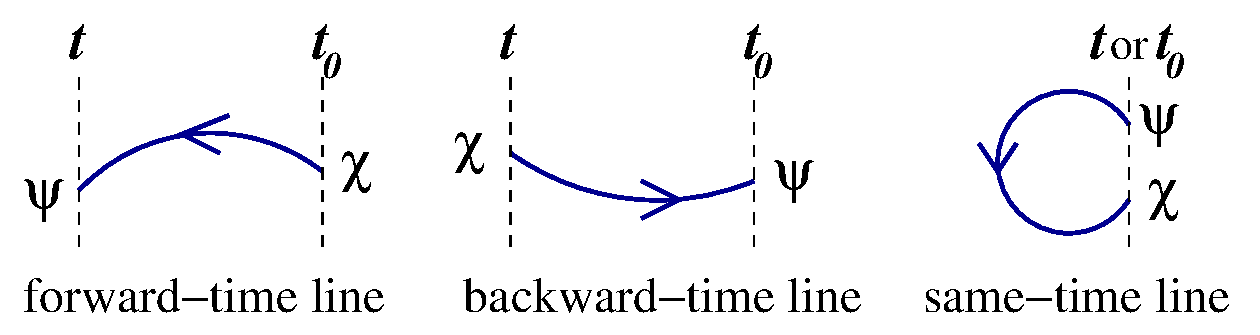
\includegraphics[width=6in]{figures/quarklines.pdf}
    \caption[The three types of quark lines that occur by integrating the quark fields when evaluating two-point temporal correlators.]{The three types of quark lines that occur by integrating the quark fields when evaluating two-point temporal correlators. Figure taken from Ref.~\cite{spectroscopy}.}
    \label{fig:quark_lines}
\end{figure}
\section{Motivating the Need for Stochastically Estimated All-to-All Propagators}
A single-hadron operator of definite momentum (consider $\bs p = 0$ without loss of generality) is a Fourier transform involving a summation over all spatial sites:
\begin{equation}
    \mathcal{O}(\boldsymbol{p}= 0, t)=\frac{1}{V} \sum_{\boldsymbol{x}} \varphi(\boldsymbol{x}, t),
\end{equation}
where $\varphi(\bs x, t)$ is a single-hadron operator located at a spatial site $\bs x$ at time $t$ and $V$ is the spatial volume of the lattice. A two-point correlator for such a hadron has the form
\begin{equation}
    C(t) = \frac{1}{V^2} \sum_{\bs x, \bs y} \bra 0\varphi(\bs x, t+t_0)\overline\varphi(\bs y, t_0) \ket 0.
\end{equation}
Calculating such a correlator appears to involve evaluating quark propagators from all spatial sites $\bs x$ to all spatial sites $\bs y$, which is an expensive computation. These are known as \emph{all-to-all} propagators. A trick can be used to avoid this by exploiting translational invariance to remove one of the spatial sums, giving
\begin{equation}
    C(t) = \frac{1}{V} \sum_{\bs x} \bra 0 \varphi(\bs x, t+t_0) \overline\varphi(0, t_0) \ket 0.
\end{equation}
Now we are tasked with evaluating the quark propagator from one single site (the origin) to all spatial site, which is a much easier task. These propagators are known as \emph{point-to-all} propagators.

Unfortunately, we cannot use this translational invariance trick in all cases. Many of our calculations necessitate the use of multi-hadron correlators (for example, if we wish to study resonances). If we consider a two-hadron operator with zero total momentum and back-to-back constituent momentum, such an operator has the form
\begin{equation}
    \mathcal{O}_{1}(\boldsymbol{p}, t) \mathcal{O}_{2}(-\boldsymbol{p}, t)=\frac{1}{V^{2}} \sum_{\boldsymbol{x}, \boldsymbol{y}} \varphi_{1}(\boldsymbol{x}, t) \varphi_{2}(\boldsymbol{y}, t) e^{-i \boldsymbol{p}(\boldsymbol{x}-\boldsymbol{y})}.
\end{equation}
When forming a two-point correlator with such an operator, we can no longer exploit translational variance to remove the need of calculating all-to-all propagators.

Additionally, calculations involving disconnected diagrams (such isoscalar meson correlators) are not amenable to point-to-all methods. Many calculations in the past have neglected contributions from disconnected diagrams, but such calculations ignore important sea quark effects which have a demonstrable effect on the resulting spectrum. There is therefore a need for a method that can efficiently calculate all-to-all propagators.
\section{Stochastically Estimating the Quark Propagator}
Since calculating Dirac matrix inverses is just an intermediate step in a larger Monte Carlo calculation, the accuracy of which is determined by the uncertainty in sampling over the gauge fields, it is unnecessary to calculate these inverses exactly. We can instead use Monte Carlo subsampling, or Monte Carlo within Monte Carlo, to stochastically estimate the quark propagators on each gauge configuration. Consider an $N\times N$ complex matrix $M$ whose inverse we wish to stochastically estimate, and a random noise vector $\eta$ whose expectations satisfy $E(\eta_i) = 0$ and $E(\eta_i \eta_j^*) = \delta_{ij}$. Assume that for any $\eta$ we can solve (say, by some variation of the conjugate gradient method) $MX=\eta$ for $X$. Then $X=M^{-1}\eta$ and
\begin{equation}
    E\left(X_{i} \eta_{j}^{*}\right)=E\left(\sum_{k} M_{i k}^{-1} \eta_{k} \eta_{j}^{*}\right)=\sum_{k} M_{i k}^{-1} E\left(\eta_{k} \eta_{j}^{*}\right)=\sum_{k} M_{i k}^{-1} \delta_{k j}=M_{i j}^{-1}.
\end{equation}
We can then in principle obtain a Monte Carlo estimate of $M^{-1}_{ij}$ by sampling over $N_R$ random noise vectors:
\begin{equation}
    M_{i j}^{-1} \approx \lim _{N_{R} \rightarrow \infty} \frac{1}{N_{R}} \sum_{r=1}^{N_{R}} X_{i}^{(r)} \eta_{j}^{(r) *}, \quad \text { where } M X^{(r)}=\eta^{(r)}.
\end{equation}
In practice, the variances that result in estimating Dirac matrix inverses in this way are too large to be useful. Notice that the above estimate only becomes exact in the limit of $N_R\rightarrow \infty$ which requires the computation of an infinite amount of solution vectors, whereas we can achieve an exact result by only solving $N$ linear systems. A technique known as \emph{dilution}~\cite{Foley:2005ac,Bernardson:1993he,Wilcox:1999ab} can tackle this issue by guaranteeing that the $M^{-1}$ is solved exactly in the limit $N_R\rightarrow N$. The maximal dilution strategy proceeds as follows: Decompose a noise vector $\eta^{(r)}$ into a sum of vectors $\eta^{(r)[s]}$ whose components are all zero except for the $s^{\rm{th}}$ component, that is,
\begin{equation}
    \eta_{j}^{(r)}=\sum_{s=1}^{N} \eta_{j}^{(r)[s]}, \quad \eta_{j}^{(r)[s]}=\eta_{j}^{(r)} \delta_{j s} \quad(\text { no sum over } j).
\end{equation}
Therefore, defining $X^{(r)[s]}$ to be the solution of $M X^{(r)[s]} = \eta^{(r)[s]}$,
\begin{equation}\
    \begin{aligned}
    \sum_{s=1}^{N} X_{i}^{(r)[s]} \eta_{j}^{(r)[s] *} &=\sum_{s} M_{i s}^{-1} \eta_{s}^{(r)} \eta_{j}^{(r)[s] *} \\
    &=\sum_{s} M_{i s}^{-1} \eta_{s}^{(r)} \eta_{j}^{(r) *} \delta_{s j}\\
    &=M_{i j}^{-1} \eta_{j}^{(r)} \eta_{j}^{(r) *}, \quad(\text { no sum over } j).
\end{aligned}
\end{equation}
If we choose noise vectors that are guaranteed to have unit modulus (such as $Z_2$, $Z_4$ or U(1) noise vectors), then it is evident that only one noise vector is needed, and $M^{-1}$ can be determined exactly by solving $N$ systems.

This maximal dilution strategy solves $M^{-1}$ exactly, but requires the solution and storage of $N$ solution vectors, so it is no more feasible than computing the inverse outright. However, it suggests that weaker dilution schemes may greatly reduce the variance, and this is shown to be the case in Ref.~\cite{Morningstar:2011ka}. Diluting a noise vector is simply the application of projection matrices onto the noise vector, i.e.\
\begin{equation}
    \eta^{[a]} = P^{(a)} \eta,
\end{equation}
where $\eta$ is a noise vector and $P^{(a)}$ is a projection matrix. Maximal dilution corresponds to $N$ such matrices (think for example of the projectors $\vb e_i \otimes \vb e_i$ in the standard basis) and solves the system exactly, but weaker dilution schemes contain fewer projections, speeding up computation at the cost of increasing variance. In general, any complete set of projection matrices $P^{(a)}$ can be used to define a dilution scheme. Observe that
\begin{equation}
\begin{aligned} M_{i j}^{-1} &=M_{i k}^{-1} \delta_{k j}=\sum_{a} M_{i k}^{-1} P_{k j}^{(a)}=\sum_{a} M_{i k}^{-1} P_{k k^{\prime}}^{(a)} P_{k^{\prime} j}^{(a)} \\ &=\sum_{a} M_{i k}^{-1} P_{k k^{\prime}}^{(a)} \delta_{k^{\prime} j^{\prime}} P_{j^{\prime} j}^{(a)}=\sum_{a} M_{i k}^{-1} P_{k k^{\prime}}^{(a)} E\left(\eta_{k^{\prime}} \eta_{j^{\prime}}^{\prime \prime}\right) P_{j^{\prime} j}^{(a)} \\ &=\sum_{a} M_{i k}^{-1} E\left(P_{k k^{\prime}}^{(a)} \eta_{k^{\prime}} \eta_{j^{\prime}}^{*} P_{j^{\prime} j}^{(a)}\right). \end{aligned}
\end{equation}
Define
\begin{equation}
    \begin{aligned}
    \eta_{k}^{[a]}&=P_{k k^{\prime}}^{(a)} \eta_{k^{\prime}},\\
    \eta_{j}^{[a] *}&=\eta_{j^{\prime}}^{*} P_{j^{\prime} j}^{(a)}=P_{j j^{\prime}}^{(a) *} \eta_{j^{\prime}}^{*},
    \end{aligned}
\end{equation}
and define $X^{[a]}$ as the solution of
\begin{equation}
    M_{i k} X_{k}^{[a]}=\eta_{i}^{[a]}.
\end{equation}
From this, we find an expression for $M^{-1}$ that can be used to calculate a Monte Carlo estimate:
\begin{equation}
    M_{i j}^{-1}=\sum_{a} M_{i k}^{-1} E\left(\eta_{k}^{[a]} \eta_{j}^{[a] *}\right)=\sum_{a} E\left(X_{i}^{[a]} \eta_{j}^{[a] *}\right).
\end{equation}
For $Z_n$ or $U(1)$ noise vectors,
\begin{equation}
    V\left(\operatorname{Re}\left(\eta_{i} \eta_{j}^{*}\right)\right)=V\left(\operatorname{Im}\left(\eta_{i} \eta_{j}^{*}\right)\right)=\frac{1}{2}\left(1-\delta_{i j}\right),
\end{equation}
where $V$ denotes the variance. This give zero variance for the diagonal elements, but introduces variance for the off-diagonal elements. Dilution, on the other hand, guarantees zero variance for many of the off-diagonal terms. Observe that
\begin{equation}
    \eta_{k} \eta_{j}^{*}=\delta_{k k^{\prime}} \eta_{k^{\prime}} \eta_{j^{\prime}}^{*} \delta_{j^{\prime} j}=\sum_{a b} P_{k k^{\prime}}^{(a)} \eta_{k^{\prime}} \eta_{j^{\prime}}^{*} P_{j^{\prime} j}^{(b)}=\sum_{a b} \eta_{k}^{[a]} \eta_{j}^{[b] *} \neq  \sum_{a} \eta_{k}^{[a]} \eta_{j}^{[a] *},
\end{equation}
but
\begin{equation}
    E\left(\eta_{k} \eta_{j}^{*}\right)=\sum_{a} E\left(\eta_{k}^{[a]} \eta_{j}^{[a] *}\right),\; \text{since}\; P^{(a)} P^{(b)}=\delta^{a b} P^{(a)}.
\end{equation}
Clearly,
\begin{equation}
    V\left(\eta_k \eta_j^*\right) = V\left(\sum_{ab}\eta_k^{[a]} \eta_j^{[b]*}\right) = \sum_{ab}V\left(\eta_k^{[a]} \eta_j^{[b]*}\right) \geq V\left(\sum_{a}\eta_k^{[a]} \eta_j^{[b]*}\right).
\end{equation}
\subsection{Application to Quark Lines}
We wish to stochastically estimate a quark line
\begin{equation}
    Q_{j k}=D_{j} \mathcal{S} \Omega^{-1} \mathcal{S} D_{k}^{\dagger}.
\end{equation}
We introduce noise vectors (having spin, color, space, and time indices) satisfying
\begin{equation}
    E(\eta)=0, \quad E\left(\eta \eta^{\dagger}\right)=I,
\end{equation}
where $I$ is the identity matrix. Inserting the identity into the expression for $Q_{jk}$ gives
\begin{equation}
    \begin{aligned}
        Q_{j k} &=D_{j} \mathcal{S} \Omega^{-1} E\left(\eta \eta^{\dagger}\right) \mathcal{S} D_{k}^{\dagger} \\
        &=E\left(D_{j} \mathcal{S} \Omega^{-1} \eta\left(D_{k} \mathcal{S} \eta\right)^{\dagger}\right),
        \end{aligned}
\end{equation}
using the hermiticity of $\mathcal S$. Defining
\begin{equation}
    \Omega \phi=\eta
\end{equation}
gives
\begin{equation}
    \begin{aligned}
        Q_{j k} &=E\left(D_{j} \mathcal{S} \phi\left(D_{k} \mathcal{S} \eta\right)^{\dagger}\right) \\
        &=E\left(\phi_{j} \eta_{k}^{\dagger}\right),
        \end{aligned}
\end{equation}
where
\begin{equation}
    \eta_{j}=D_{j} \mathcal{S} \eta\quad \text{and}\quad \phi_{j}=D_{j} \mathcal{S} \phi.
\end{equation}
This reveals a great advantage of this method: the quark lines factor into outer products of source vectors and sink vectors. This will allow us to fully construct the source and sinks separately, and then combine them to form various single- and multi-hadron correlators. More will be said about this shortly.

To reduce variance via noise dilution, we consider a complete set of dilution projectors $P^{(a)}$ which are indexed by spin, color, space, and time as follows,
\begin{equation}
    \begin{aligned}
        Q_{j k} &=\sum_{a} D_{j} \mathcal{S} \Omega^{-1} P^{(a)} P^{(a) \dagger} \mathcal{S} D_{k}^{\dagger} \\
        &=\sum_{a} D_{j} \mathcal{S} \Omega^{-1} P^{(a)} E\left(\eta \eta^{\dagger}\right) P^{(a) \dagger} \mathcal{S} D_{k}^{\dagger} \\
        &=\sum_{a} E\left(D_{j} \mathcal{S} \Omega^{-1} P^{(a)} \eta\left(D_{k} \mathcal{S} P^{(a)} \eta\right)^{\dagger}\right)\\
        &=\sum_{a} E\left(\phi_{j}^{[a]} \eta_{k}^{[a] \dagger}\right),
    \end{aligned}
\end{equation}
where we have defined
\begin{equation}
    \begin{aligned}
        \eta_{j}^{[a]} &=D_{j} \mathcal{S} \eta^{[a]}, & \eta^{[a]} &=P^{(a)} \eta \\
        \phi_{j}^{[a]} &=D_{j} \mathcal{S} \phi^{[a]}, & \Omega \phi^{[a]} &=\eta^{[a]}.
    \end{aligned}
\end{equation}
Since we use LapH-smeared quark fields, we are motivated to introduce noise vectors $\rho$ only in the LapH subspace (the vector space spanned by the lowest $N$ eigenvectors of the gauge-covariant Laplacian) which are indexed only by spin, time, and Laplacian eigenmode number, rather than noise vectors in the full spin/color/space/time vector space. Ref.~\cite{Morningstar:2011ka} demonstrates a significant cost reduction in doing so. The process of stochastically estimating quark lines by introducing diluted noise vectors only in the LapH subspace is known as the \emph{stochastic LapH} method. Explicitly, we can evaluate a forward-time quark line as follows:
\begin{equation}
    \begin{aligned}
    Q_{j k} &=D_{j} \mathcal{S} \Omega^{-1} \mathcal{S} D_{k}^{\dagger} \\
    &=D_{j} \mathcal{S} \Omega^{-1} V_{s} V_{s}^{\dagger} D_{k}^{\dagger} \\
    &=\sum_{a} D_{j} \mathcal{S} \Omega^{-1} V_{s} P^{(a)} P^{(a) \dagger} V_{s}^{\dagger} D_{k}^{\dagger} \\
    &=\sum_{a} D_{j} \mathcal{S} \Omega^{-1} V_{s} P^{(a)} E\left(\rho \rho^{\dagger}\right) P^{(a) \dagger} V_{s}^{\dagger} D_{k}^{\dagger} \\
    &=\sum_{a} E\left(D_{j} \mathcal{S} \Omega^{-1} V_{s} P^{(a)} \rho\left(D_{k} V_{s} P^{(a)} \rho\right)^{\dagger}\right),
    \end{aligned}
\end{equation}
where $V$ a matrix whose columns are the $N$ lowest eigenvectors of the gauge-covariant Laplacian. We then define the displaced-smeared-diluted source and sink vectors by
\begin{equation}
    \begin{array}{ll}
        \varrho_{j}^{[a]}=D_{j} V_{s} \varrho, & \varrho^{[a]}=P^{(a)} \rho \\
        \varphi_{j}^{[a]}=D_{j} \mathcal{S} \varphi^{[a]}, & \Omega \varphi^{[a]}=V_{s} \varrho^{[a]},
        \end{array}
\end{equation}
giving
\begin{equation}\label{eq:Qjk}
    Q_{j k}=\sum_{a} E\left(\varphi_{j}^{[a]} \varrho_{k}^{[a] \dagger}\right).
\end{equation}
\subsection{Correlator Factorization}
An important result of this stochastic method is that correlators end up factorizing into various combinations of source and sink vectors. We can see this by considering a baryon-baryon correlator as an example to sketch out this process. A correlation matrix for baryons can be written as (c.f. Ch.~\ref{ch:operators}),
\begin{equation}
    C_{l \overline{l}}\left(t_{F}-t_{0}\right)=\left\langle B_{l}\left(t_{F}\right) \overline{B}_{\overline{l}}\left(t_{0}\right)\right\rangle,
\end{equation}
where $l$ and $\overline l$ are compound indices labeling the quantum numbers of interest. In practice, we average over all source times $t_0$ for increased statistics. In terms of our elemental baryon operators and the projection coefficients, we can write this as
\begin{equation}
    \begin{aligned}
    C_{l \overline{l}}\left(t_{F}-t_{0}\right)=&c_{\alpha \beta \gamma}^{(l)} c_{\overline{\alpha} \overline{\beta} \overline{\gamma}}^{(\overline{l}) *}\left\langle\Phi_{\alpha \beta \gamma}^{A B C}\left(t_{F}\right) \overline{\Phi}_{\overline{\alpha} \overline{\beta} \overline{\gamma}}^{\overline{A B C}}\left(t_{0}\right)\right\rangle \\
    =&c_{\alpha \beta \gamma}^{(l)} c_{\overline{\alpha} \overline{\beta} \overline{\gamma}}^{(\overline{l}) *} \sum_{\boldsymbol{x} \overline{\boldsymbol{x}}} \varepsilon_{a b c} \varepsilon_{\overline{a} \overline{b} \overline{c}} e^{-i \boldsymbol{p} \cdot(\boldsymbol{x}-\overline{\boldsymbol{x}})}\\
    &\times\left\langle q_{a \alpha}^{A}\left(\boldsymbol{x}, t_{F}\right) q_{b \beta}^{B}\left(\boldsymbol{x}, t_{F}\right) q_{c \gamma}^{C}\left(\boldsymbol{x}, t_{F}\right)\right.\\
    &\qquad\left.\times \overline{q}_{\overline{c \gamma}}^{\overline{C}}\left(\overline{\boldsymbol{x}}, t_{0}\right) \overline{q}_{\overline{b} \beta}^{\overline{B}}\left(\overline{\boldsymbol{x}}, t_{0}\right) \overline{q}_{\overline{a} \overline{\alpha}}^{\overline{A}}\left(\overline{\boldsymbol{x}}, t_{0}\right)\right\rangle,
    \end{aligned}
\end{equation}
where the $l$ and $\overline l$ have the same three-momentum $\bs p$. Computing the path integral over the Grassmann fields yields the following sum over various products of quark lines (i.e.\ the Wick contractions),
\begin{eqnarray*}
&&C_{l\overline{l}}(t)
= c^{(l)}_{\alpha\beta\gamma}
c^{(\overline{l})\ast}_{
\overline{\alpha}\overline{\beta}\overline{\gamma}}
\sum_{\bs{x}\overline{\bs{x}}}\ \varepsilon_{abc}
\   \varepsilon_{\overline{a}\overline{b}\overline{c}} 
e^{-i\bs{p}\cdot(\bs{x}-\overline{\bs{x}})}\  \nonumber\\
&\times& \Bigl\langle {\cal Q}^{(A\overline{A})}_{
a\alpha ;\overline{a}\overline{\alpha}}
{\cal Q}^{(B\overline{B})}_{b\beta ;\overline{b}\overline{\beta}}
{\cal Q}^{(C\overline{C})}_{c\gamma ;\overline{c}\overline{\gamma}}
-{\cal Q}^{(A\overline{A})}_{a\alpha;\overline{a}\overline{\alpha}}
{\cal Q}^{(B\overline{C})}_{b\beta   ;\overline{c}\overline{\gamma}}
{\cal Q}^{(C\overline{B})}_{c\gamma ;\overline{b}\overline{\beta}}
\nonumber\\
&-&{\cal Q}^{(A\overline{B})}_{a\alpha;\overline{b}\overline{\beta}}
{\cal Q}^{(B\overline{A})}_{b\beta  ;\overline{a}\overline{\alpha}}
{\cal Q}^{(C\overline{C})}_{c\gamma ;\overline{c}\overline{\gamma}}
- {\cal Q}^{(A\overline{C})}_{a\alpha;\overline{c}\overline{\gamma}}
{\cal Q}^{(B\overline{B})}_{b\beta ;\overline{b}\overline{\beta}}
{\cal Q}^{(C\overline{A})}_{c\gamma ;\overline{a}\overline{\alpha}}
\nonumber\\
&+&
{\cal Q}^{(A\overline{C})}_{a\alpha;\overline{c}\overline{\gamma}}
{\cal Q}^{(B\overline{A})}_{b\beta ;\overline{a}\overline{\alpha}}
{\cal Q}^{(C\overline{B})}_{c\gamma ;\overline{b}\overline{\beta}}
+{\cal Q}^{(A\overline{B})}_{a\alpha;\overline{b}\overline{\beta}}
{\cal Q}^{(B\overline{C})}_{b\beta ;\overline{c}\overline{\gamma}}
{\cal Q}^{(C\overline{A})}_{c\gamma ;\overline{a}\overline{\alpha}}
\Bigr\rangle_U,
\end{eqnarray*}
where we have defined $t\equiv t_F - t_0$, where time and spacial labels have been omitted, and where
\begin{equation}
    \langle f(U)\rangle_{U}=\frac{\int \mathcal{D} U f(U) \operatorname{det}(M[U]) e^{-S_{G}[U]}}{\int D U \operatorname{det}(M[U]) e^{-S_{G}[U]}}.
\end{equation}
This expression is depicted diagramatically in Fig.~\ref{fig:baryon_corr}.

Using Eq.~(\ref{eq:Qjk}), we can dramatically simplify the above expression for $C_{l\overline l}(t)$. Let us first define the following quantity,
\begin{equation}\label{eq:baryon_func}
    \begin{array}{l}
        \mathcal{B}_{l}^{\left[b_{1} b_{2} b_{3}\right]}\left(\varphi_{1}, \varphi_{2}, \varphi_{3} ; t\right)=c_{\alpha \beta \gamma}^{(l)} \sum_{x} e^{-i p \cdot x} \varepsilon_{a b c} \\
        \quad \times \varphi_{a \alpha x t}^{\left[b_{1}\right]}\left(\rho_{1}\right) \varphi_{b \beta x t}^{[b]}\left(\rho_{2}\right) \varphi_{c \gamma x t}^{\left[b_{3}\right]}\left(\rho_{3}\right),
        \end{array}
\end{equation}
where $b_1$, $b_2$, and $b_3$ are dilution indices, and we use a short-hand notation to denote $\varphi_k = \varphi(\rho_k)$, i.e.\ the sink vector corresponding to the noise vector $\rho_k$. The baryon correlator matrix element is then given by,
\begin{equation}\label{eq:corr_fac}
    \begin{aligned}
        C_{l \overline{l}}\left(t_{F}-t_{0}\right) &=\left\langle\mathcal{B}_{l}^{\left[b_{1} b_{2} b_{3}\right]}\left(\varphi_{1}, \varphi_{2}, \varphi_{3} ; t_{F}\right)\right.\\
        & \times\left(\delta_{A B C}^{\overline{A B C}} \mathcal{B}_{l}^{\left[b_{1} b_{2} b_{3}\right]}\left(\varrho_{1}, \varrho_{2}, \varrho_{3} ; t_{0}\right)\right.\\
        &-\delta_{A B C}^{\overline{A C B}} \mathcal{B}_{l}^{\left[b_{1} b_{3} b_{2}\right]}\left(\varrho_{1}, \varrho_{3}, \varrho_{2} ; t_{0}\right) \\
        &-\delta_{A B C}^{\overline{B A C}} \mathcal{B}_{\overline{l}}^{\left[b_{2} b_{1} b_{3}\right]}\left(\varrho_{2}, \varrho_{1}, \varrho_{3} ; t_{0}\right) \\
        &-\delta_{A B C}^{\overline{C B A}} \mathcal{B}_{\overline{l}}^{\left[b_{3} b_{2} b_{1}\right]}\left(\varrho_{3}, \varrho_{2}, \varrho_{1} ; t_{0}\right) \\
        &+\delta_{A B C}^{\overline{C A B}} \mathcal{B}_{\overline{l}}^{\left[b_{2} b_{3} b_{1}\right]}\left(\varrho_{2}, \varrho_{3}, \varrho_{1} ; t_{0}\right) \\
        &\left.\left.+\delta_{A B C}^{\overline{B C A}} \mathcal{B}_{\overline{l}}^{\left[b_{3} b_{1} b_{2}\right]}\left(\varrho_{3}, \varrho_{1}, \varrho_{2} ; t_{0}\right)\right)^{*}\right\rangle_{U, \rho},
    \end{aligned}
\end{equation}
where $\delta_{A B C}^{D E F}=\delta_{A D} \delta_{B E} \delta_{C F}$ and $\langle\ldots\rangle_{U, \rho}$ denotes an expectation value over the gauge fields $U$ and the noise vectors $\rho_k$.

This factorization process is significant because it allows us to calculate the source and sinks separately and store the results on disk to be later combined to construct the correlators we wish to study, which is particularly advantageous for when we want to study large correlation matrices.
\begin{figure}
    \centering
    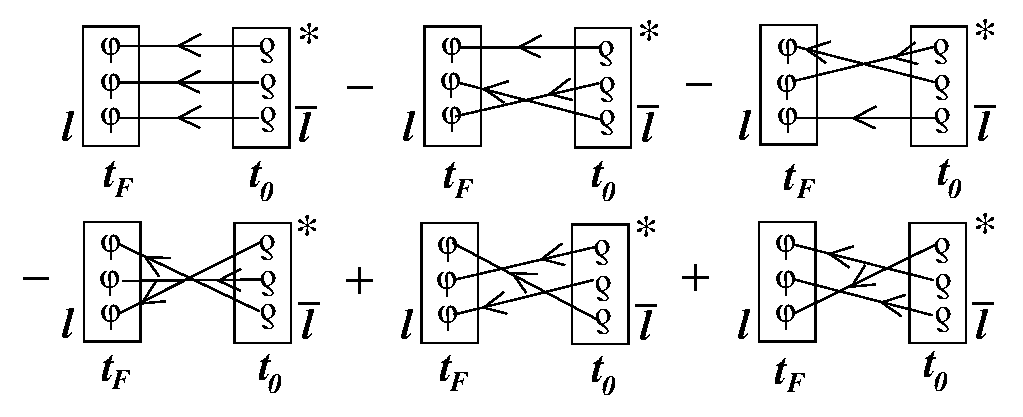
\includegraphics[width=6in]{figures/baryon_corr_diag.pdf}
    \caption[A diagrammatic representation of Eq.~(\ref{eq:corr_fac}) for a baryon correlator with source time $t_0$ and later sink time $t_F$.]{A diagrammatic representation of Eq.~(\ref{eq:corr_fac}) for a baryon correlator with source time $t_0$ and later sink time $t_F$. The boxes represent the baryon functions defined in Eq.~(\ref{eq:baryon_func}) with the first quark at the top of each box. Lines connecting a $\varrho$ to a $\varphi$ denote a summation over dilution indices. The same noise is used for both ends of any single line, and different lines use different noises. An asterisk denotes complex conjugation. Figure taken from Ref.~\cite{spectroscopy}.}
    \label{fig:baryon_corr}
\end{figure}